\documentclass[12pt, leqno]{article}

\usepackage[utf8]{inputenc}
\usepackage[T1]{fontenc}
\usepackage{polski}

\usepackage[fleqn]{amsmath}
\usepackage{graphicx}
\usepackage[fleqn]{mathtools}
\usepackage{algorithm}
\usepackage{amssymb} % real numbers symbol

\usepackage{ulem} % page numbering

\usepackage{titlesec}
\newcommand{\sectionbreak}{\clearpage} % new page before new section

\usepackage[labelformat=empty]{caption}
\usepackage[margin=1in, top=0.75in]{geometry}
 
\title{
    \Huge \textbf{Raport - temat 2} \linebreak
    \\[2pt]
    \LARGE 
    \uline{Interpolacja.} \\[5mm]
    Zadanie 20 
}
\date{31.10.2018}
\author{Przemysław Wiczołek \\ gr. F3}

\begin{document}
    \pagenumbering{gobble} % skip site number
    \maketitle
    \newpage
    \pagenumbering{arabic}
    \titlelabel{\thetitle.\quad} % dot after section number

    \section{Wstęp teoretyczny}
        \paragraph{Treść zadania:}
        \textit{Interpolacja funkcjami kwadratowymi na obszarze $D: |x|+|y| \leq 1$ podzielonym na $4n^2$
        trójkątów przystających. Tablicowanie funkcji, przybliżenia i błędu w środkach ciężkości trójkątów.
        Obliczenie błędu średniokwadratowego w tych punktach.} \\[5mm]
        Postać wielomianu interpolacyjnego stopnia drugiego dla funkcji 2 zmiennych to:
        \[ p(x,y) = a_0 + a_1x + a_2y + a_3xy + a_4x^2 + a_5y^2 \]
        Niech $(x_0, y_0),\: (x_1, y_1),\: (x_2, y_2)$ będą współrzędnymi danego trójkąta, wówczas\\[2mm]
        $(x_3, y_3) = $ {\large $(\frac{x_0 + x_1}{2}, \frac{y_0 + y_1}{2}),\:$}
        $(x_4, y_4) = $ {\large $(\frac{x_0 + x_2}{2}, \frac{y_0 + x_2}{2}),\:$}
        $(x_5, y_5) = $ {\large $(\frac{x_1 + x_2}{2}, \frac{y_1 + y_2}{2})$} \\[2mm] 
        to współrzędne środków jego boków.\\[3mm]
        Żeby obliczyć współczynniki p(x,y) rozwiązujemy układ 6 równań:
        \[
        \begin{cases}
            p(x_0, y_0) = a_0 + a_1x_0 + a_2y_0 + a_3x_0y_0 + a_4{x_0}^2 + a_5{y_0}^2 = f(x_0, y_0) &\\
            p(x_1, y_1) = a_0 + a_1x_1 + a_2y_1 + a_3x_1y_1 + a_4{x_1}^2 + a_5{y_1}^2 = f(x_1, y_1) &\\
            p(x_2, y_2) = a_0 + a_1x_2 + a_2y_2 + a_3x_2y_2 + a_4{x_2}^2 + a_5{y_2}^2 = f(x_2, y_2) &\\
            p(x_3, y_3) = a_0 + a_1x_3 + a_2y_3 + a_3x_3y_3 + a_4{x_3}^2 + a_5{y_3}^2 = f(x_3, y_3) &\\
            p(x_4, y_4) = a_0 + a_1x_4 + a_2y_4 + a_3x_4y_4 + a_4{x_4}^2 + a_5{y_4}^2 = f(x_4, y_4) &\\
            p(x_5, y_5) = a_0 + a_1x_5 + a_2y_5 + a_3x_5y_5 + a_4{x_5}^2 + a_5{y_5}^2 = f(x_5, y_5) &\\
        \end{cases}
        \]
        gdzie \textit{f} to interpolowana funkcja.\\[3mm]
        Podany obszar \textit{D} dzielimy na $4n^2$ przystających 
        trójkątów prostokątnych.\\
        Dla każdego z małych trójkątów rozwiązujemy podany wyżej układ równań i obliczamy 
        wartość wielomianu \textit{p} oraz funkcji f w środku ciężkości tego trójkąta:
        {\large $(\frac{x_0 + x_1 + x_2}{3}, \frac{y_0 + y_1 + y_2}{3})$}. Następnie obliczamy wartość 
        błędu względnego w tym punkcie.\\[3mm]
        Błąd średniokwadratowy obliczamy ze wzoru:
        \[
            MSE(\theta) = \sum\limits_{i=1}^{4n^2} (f(\theta_i) - p(\theta_i))^2,\quad 
            \theta = {\theta_1, ... , \theta_{4n^2}}
        \]
        gdzie $\theta_i$ to współrzędne środka ciężkości i-tego trójkąta.

    \section{Opis metody}
            \subsection*{Implementacja}
            Implementacja została przeprowadzona poprzez funkcję
            \[ [meanSquaredError,\; valuesArray] = squarePolynInterpol(func,\; n)\]
            \subsection*{Podział na trójkąty}
            \begin{algorithm} 
                \vspace{2mm}
                \begin{enumerate}
                \item{Zaczynamy od pierwszego małego trójkąta o współrzędnych $(0,0),\; (\frac{1}{n}, 0),\; 
                    (0, \frac{1}{n})$\\ w I ćwiartce układu kartezjańskiego.}
                \item{Odbijamy go w pozostałych ćwiartkach układu współrzędnych.}
                \item{Obliczamy trójkąt przeciwległy, symetryczny względem przeciwprostokątnej poprzez 
                      dodanie $(\frac{1}{n}, \frac{1}{n})$ do punktu przy kącie prostym.}
                \item{Odbijamy drugi trójkąt w pozostałych ćwiartkach.}
                \item{Przechodzimy do następnego trójkąta poprzez dodanie $\frac{1}{n}$ do pierwszej
                      współrzędnej każdego punktu.}
                \item{Powtarzamy powyższą procedurę aż dojdziemy do ostatniego trójkąta w pierwszym wierszu, 
                    dla którego nie ma przeciwległego.} 
                \item{Przechodzimy do początku następnego wiersza poprzez dodanie $\frac{1}{n}$ do drugiej
                      współrzędnej każdego punktu pierwszego trójkąta w aktualnym wierszu.}
                \item{Powtarzamy powyższą procedurę aż dojdziemy do ostatniego wiersza.}
                \end{enumerate}
                \vspace{2mm}
            \end{algorithm}
            Dla pierwszego wiersza będziemy mieli $n$ małych trójkątów (bez przeciwległych).
            W każdym wierszu liczba trójkątów zmniejsza się o 1, więc kolumny wystarczy iterować od\\
            $1$ do $n - aktualnyWiersz$. Przez wiersze należy przechodzić od $1$ do $n$.\\
            W ten sposób otrzymujemy cały obszar $D: |x| + |y| \leq 1$.
            \subsection*{Obliczanie współczynników wielomianu interpolacyjnego}
            Tak opisałem wcześniej, dla każdego trójkąta obliczamy kolejny wielomian interpolacyjny.
            Dla każdego punktu trójkąta $(x,y)$ przekształcamy go funkcją: 
            \[ polynomialScheme(x,y) = [1,\; x,\; y,\; x*y,\; x*x,\; y*y] \]
            w wektor, który będzie lewą stroną jednego z naszych równań.\\
            Otrzymujemy macierz $A \in \mathbb{R}^{6 \times 6}$.\\
            Z obliczenia wartości funkcji interpolowanej mamy wektor $b \in \mathbb{R}^{6}$.\\
            Rozwiązujemy układ równań liniowych $Ax = b$, gdzie otrzymany $x\in \mathbb{R}^{6}$ jest
            wektorem współczynników wielomianu interpolacyjnego.
    \section{Wyniki} 
        \vspace{-1mm}
        Odpowiednio pliki: \textit{errorGraph.m\quad timeGraph.m\quad examples.m.}
        \vspace{-2mm}
        \subsection*{Dokładność}
        \begin{figure}[!h]
            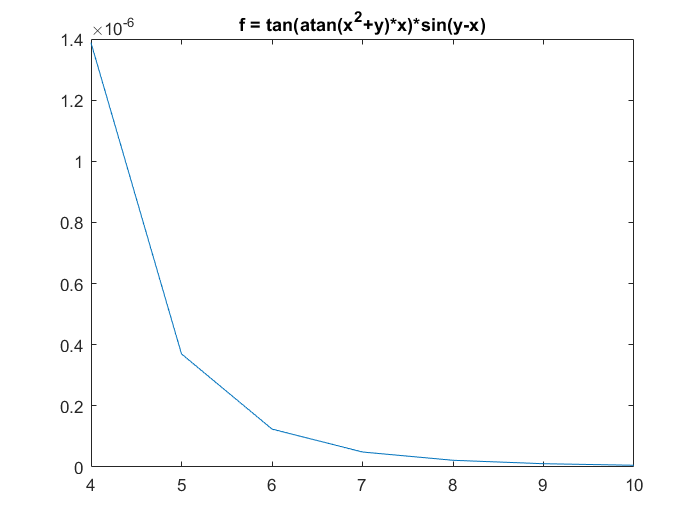
\includegraphics[width=\linewidth]{graph.png}
            \caption{Wykres błędu średniokwadratowego w zależności od $n$}
        \end{figure}
        Jak widać nawet dla dosyć skomplikowanej funkcji błąd średniokwadratowy jest niewielki i szybko
        maleje wraz ze wzrostem $n$. Mimo tego dla tej funkcji błąd względny w niektórych punktach jest
        ogromny.

        \newpage
        \subsection*{Czas}
        \begin{figure}[!h]
            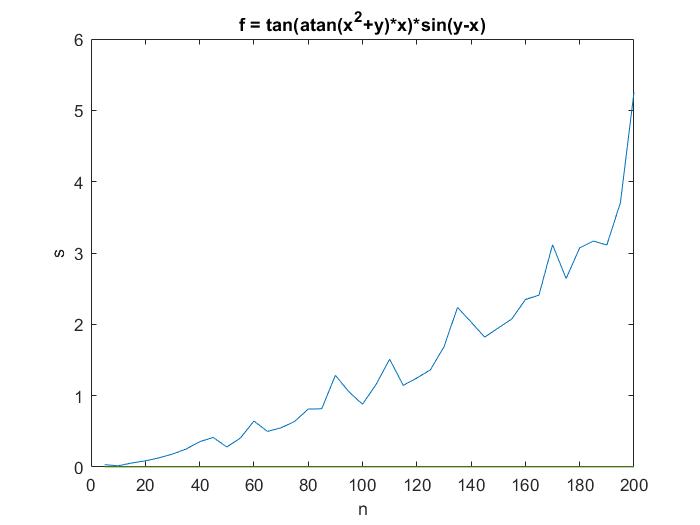
\includegraphics[width=\linewidth]{graph1.png}
            \caption{Wykres czasu w zależności od $n$}
        \end{figure}

        \newpage
        \subsection*{Przykłady obliczeniowe}
        \begin{enumerate}
            \large
            \item{$f(x, y) = \frac{1}{sin(x^2) + e^{-x^2 - y^2}}$,\quad $n = 2$}
            \begin{figure}[!h]
                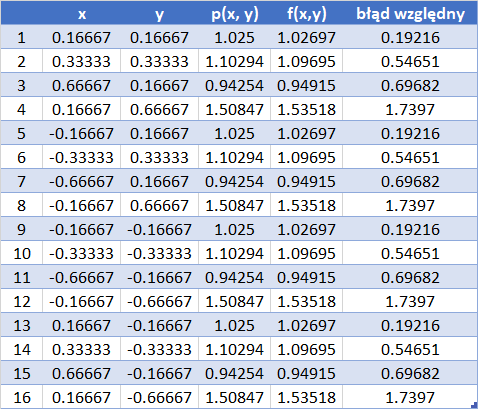
\includegraphics[width=\linewidth]{func1.png}
            \end{figure}\\
            $bladSrKwadratowy = 19.922 * 10^{-5}$

            \newpage
            \large
            \item{$f(x, y) = log(1 + (x + y)^2) - cos(\frac{x+y}{1 + (x+y)^2})$,\quad $n = 2$}
            \begin{figure}[!h]
                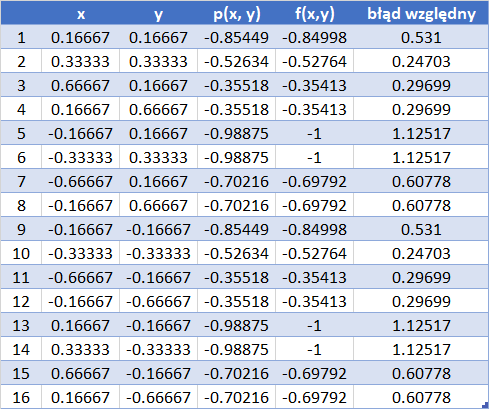
\includegraphics[width=\linewidth]{func2.png}
            \end{figure}\\
            $bladSrKwadratowy = 3.918 * 10^{-5}$

            \newpage
            \large
            \item{$f(x, y) = tan(atan(x^2 + y)*x)*sin(y-x)$,\quad $n = 2$}
            \begin{figure}[!h]
                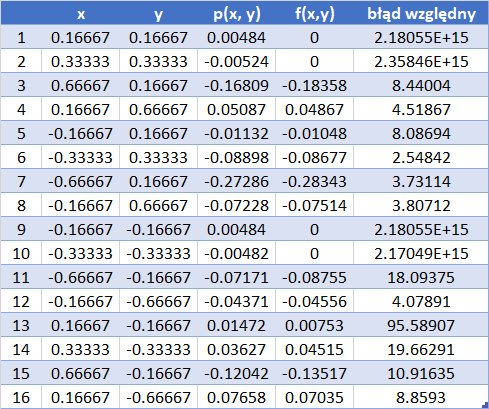
\includegraphics[width=\linewidth]{func3.png}
            \end{figure}\\
            $bladSrKwadratowy = 6.935 * 10^{-5}$

            \newpage
            \large
            \item{$f(x, y) = sin(\frac{27951}{256}*x*y)$,\quad $n = 8$}
            \begin{figure}[!h]
                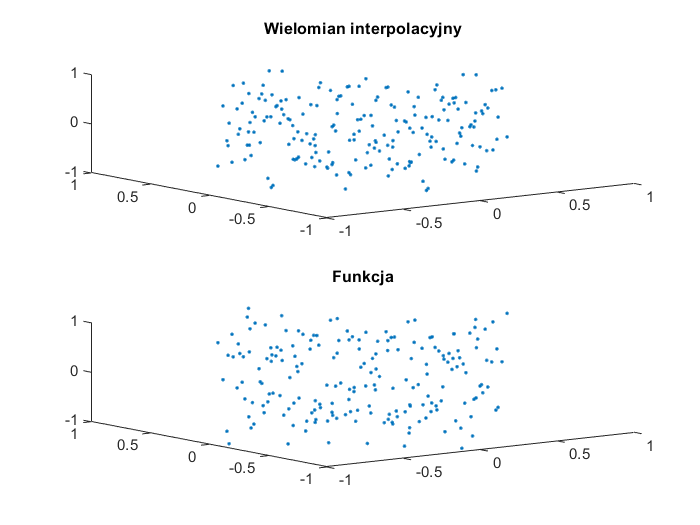
\includegraphics[width=\linewidth]{func4.png}
            \end{figure}\\
            $bladSrKwadratowy = 54689.2 * 10^{-5}$
        \end{enumerate}
    \section{Podsumowanie}
        \paragraph{}
        Reasumując powyższą analizę, interpolacja funkcji wielu zmiennych nie jest zadaniem zbyt
        trudnym obliczeniowo, jeżeli obszar interpolacji jest stosunkowo niewielki. Dla danego obszaru
        $D: |x| + |y| \leq 1$ już przy $n=2$ otrzymujemy znośną dokładność, a czas obliczania jest pomijalny.
        Gdybyśmy chcieli rozszerzyć obszar na np. $|x| + |y| \leq 10^6$ przy tym samym rozmiarze 
        trójkątów potrzeba by $n = 2*10^6$, a wówczas na obliczenia potrwały by kilka dni.
        \paragraph{}
        Kolejną rzeczą, którą należy rozważyć jest błąd względny, który w miejscach, w których funkcja
        interpolowana jest źle określona, może osiągać ogromne wartości, tak jak w trzecim przykładzie.
        Projektując ogólny algorytm ciężko jest przewidzieć, w jakich punktach interpolować, aby nie
        osiągnąć tak dużego zaburzenia.
        \paragraph{}
        Należy również zwrócić uwagę, żeby nie korzystać tylko z jednego sposobu obliczania błedu
        interpolacji. Tak jak widać w ostatnim przykładzie, pomimo ogromnych wartości błedu względnego,
        błąd średniokwadratowy jest dosyć niewielki. Użycie tylko jednego wskaźnika błędu mogłoby spowodować 
        odrzucenie sposobu interpolacji jako błędnego, mimo, że miałby po prostu inne właściwości.
\end{document}
